\documentclass[11pt]{article}

\usepackage[T1]{fontenc}
\usepackage{lmodern}
\usepackage[margin=1.1in]{geometry}
\usepackage{amsmath,amssymb}
\usepackage{booktabs}
\usepackage{array}
\usepackage{microtype}
\usepackage{xcolor}
\usepackage{graphicx}
\usepackage[font=small,labelfont=bf,width=0.95\textwidth]{caption}
\usepackage{placeins}
\usepackage[hidelinks]{hyperref}

\newcommand{\code}[1]{\texttt{\small #1}}
\setlength{\emergencystretch}{2.5em}

\title{Does the Depth Finding Survive at Eight Layers?\\
\large A CLS decomposition and attention-suppression ablation of the
\code{layers8} arm}
\author{Anthony Tong}
\date{2026-08-04}

\begin{document}
\maketitle

\begin{abstract}
The 16-layer MARINA model does almost no work in its first ten cross-attention
blocks: suppressing them costs $0.0072$ cosine, while suppressing the last block
alone costs $0.0368$. That raised an obvious question --- is the depth simply
unused, so that a shallower model would behave identically? This note answers it
by repeating the same two measurements on two independently trained 8-layer
checkpoints. The answer is that depth is \emph{not} wasted so much as
\emph{redistributed}. The number of blocks that actually carry computation is
$5$--$6$ in both models, and the work those final blocks do is quantitatively
almost identical across depths --- suppressing the last $k$ blocks costs the same
cosine at 8 layers as at 16, for every $k \le 4$, to within $0.012$. What changes
is only how many idle blocks sit in front: ten of sixteen at full depth, two or
three of eight. The modality budget is likewise depth-invariant. This is direct
mechanistic support for the retrieval result that \code{layers8} matches
\code{layers12} on \code{rank@1}.
\end{abstract}

\section{Setup}

Two measurements are repeated verbatim from the 16-layer decomposition, on
checkpoints from the depth sweep.

\begin{description}
  \item[Attribution.] The exact additive decomposition of the final CLS token
    into per-modality contributions plus an FFN, bias and initialisation
    residual. Shares sum to $1$ by construction; the reported
    \code{budget\_sums\_to} confirms closure to within $1.5\times 10^{-8}$.
  \item[Suppression.] Zeroing the cross-attention output of the first $k$ or
    last $k$ blocks and remeasuring cosine against the true fingerprint.
\end{description}

\begin{table}[htbp]
\centering
\caption{Checkpoints. The two 8-layer arms stopped at different epochs, which is
the expected behaviour for \code{val/mean\_cos} with \code{patience: 30}.}
\label{tab:ckpts}
\small
\begin{tabular}{llrrr}
\toprule
Arm & Checkpoint & Layers & $n$ molecules & Baseline cos \\
\midrule
\code{layers16} (\code{final1}) & \code{best.ckpt}            & 16 & 256 / 512 & 0.9529 / 0.9546 \\
\code{layers8-s0}               & \code{epoch\_epoch=728.ckpt} & 8  & 2048      & 0.9536 \\
\code{layers8-s1}               & \code{epoch\_epoch=631.ckpt} & 8  & 2048      & 0.9533 \\
\bottomrule
\end{tabular}
\end{table}

The 8-layer arms are measured on $2048$ molecules, the 16-layer reference on
$256$ (attribution) and $512$ (suppression). The sample sizes differ because the
16-layer numbers were reused from the earlier run rather than recomputed; this
is the main caveat and is revisited in \S\ref{sec:caveats}.

\section{Result 1: the live suffix is 5--6 blocks at either depth}

Table~\ref{tab:first} gives the cost of suppressing the first $k$ blocks. Define
the \emph{inert prefix} as the largest $k$ whose suppression costs less than
$0.01$ cosine, and the \emph{live suffix} as the remaining blocks.

\begin{table}[htbp]
\centering
\caption{Cosine drop from suppressing the first $k$ cross-attention blocks.
Dashes mark $k$ values not measured for that arm.}
\label{tab:first}
\small
\begin{tabular}{lrrrrrrrrr}
\toprule
$k$ & 1 & 2 & 3 & 4 & 5 & 6 & 8 & 10 & 12 \\
\midrule
\code{layers16}   & 0.0000 & 0.0000 & 0.0000 & 0.0000 & $-$0.0001 & 0.0002 & 0.0010 & 0.0072 & 0.2523 \\
\code{layers8-s0} & $-$0.0001 & 0.0017 & 0.0192 & 0.1443 & 0.3452 & 0.4315 & 0.7696 & --- & --- \\
\code{layers8-s1} & $-$0.0002 & 0.0007 & 0.0078 & 0.1507 & 0.3089 & 0.4222 & 0.7565 & --- & --- \\
\bottomrule
\end{tabular}
\end{table}

\begin{itemize}
  \item \code{layers16}: inert prefix $10$, live suffix $\mathbf{6}$ of 16.
  \item \code{layers8-s0}: inert prefix $2$, live suffix $\mathbf{6}$ of 8.
  \item \code{layers8-s1}: inert prefix $3$, live suffix $\mathbf{5}$ of 8.
\end{itemize}

The live suffix is the same $5$--$6$ blocks in all three checkpoints. Halving
the depth did not halve the amount of computation; it removed idle blocks.

Both depths also show a sharp cliff rather than a gradual decline --- at 16
layers between $k=10$ and $k=12$, at 8 layers between $k=3$ and $k=4$. In both
cases the cliff sits about six blocks from the end.

\FloatBarrier
\section{Result 2: the final blocks are quantitatively depth-invariant}

The stronger version of the claim is in Table~\ref{tab:last}: it is not merely
that a similar \emph{number} of blocks is live, but that they do the same
\emph{amount} of work.

\begin{table}[htbp]
\centering
\caption{Cosine drop from suppressing the last $k$ blocks. The 8- and 16-layer
columns agree to within $0.012$ for every $k \le 4$, despite a 2$\times$
difference in total depth.}
\label{tab:last}
\small
\begin{tabular}{lrrrrrr}
\toprule
$k$ & 1 & 2 & 3 & 4 & 6 & 8 \\
\midrule
\code{layers16}   & 0.0368 & 0.1133 & 0.1935 & 0.2720 & 0.4498 & 0.6829 \\
\code{layers8-s0} & 0.0392 & 0.1125 & 0.1840 & 0.2600 & 0.5402 & 0.7696 \\
\code{layers8-s1} & 0.0382 & 0.1140 & 0.1898 & 0.2605 & 0.5500 & 0.7565 \\
\midrule
max spread        & 0.0024 & 0.0015 & 0.0095 & 0.0120 & 0.1002 & 0.0867 \\
\bottomrule
\end{tabular}
\end{table}

For $k \le 4$ the three checkpoints are interchangeable. The curves separate
only at $k \ge 6$, which is exactly where the 8-layer model has run out of
blocks and is being asked to give up its inert prefix as well.

Read together with Table~\ref{tab:first}, the picture is that MARINA's
cross-attention stack does a fixed amount of work in a fixed number of blocks
at the end, and pads the front with however many identity-like blocks the
architecture provides.

\begin{figure}[htbp]
\centering
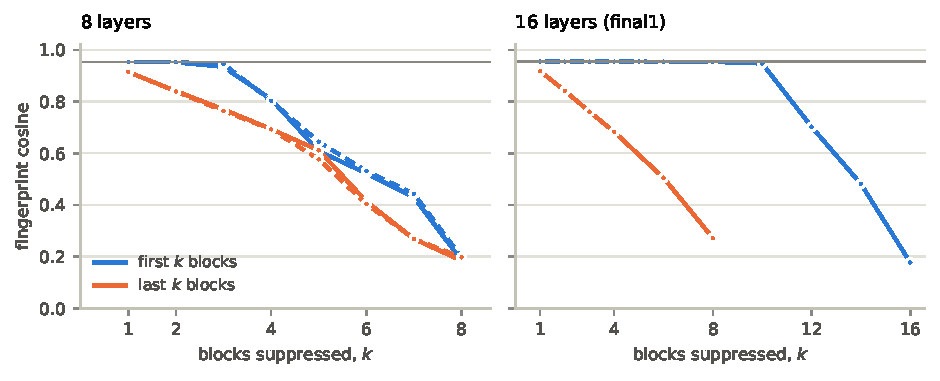
\includegraphics[width=0.92\textwidth]{fig-depth-ablation-8L.pdf}
\caption{Suppression curves at both depths. The last-$k$ curves overlie one
another; the first-$k$ curves are shifted by the difference in inert prefix.}
\end{figure}

\begin{figure}[htbp]
\centering
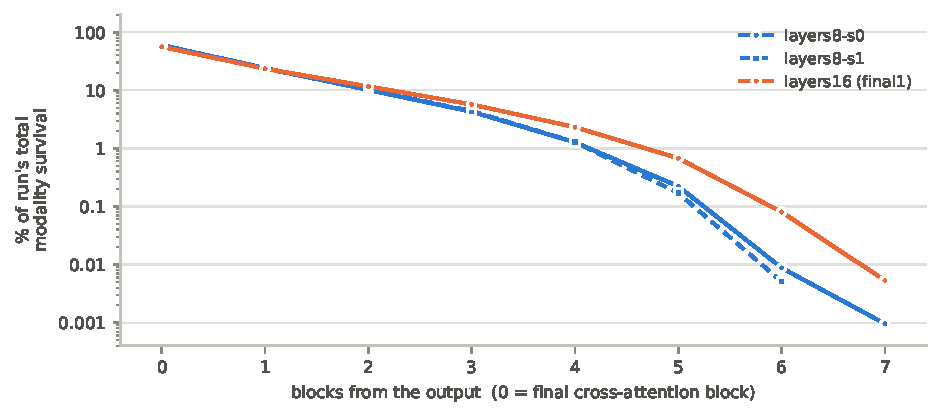
\includegraphics[width=0.92\textwidth]{fig-depth-alignment.pdf}
\caption{The same curves aligned on distance from the final block, which is the
coordinate in which they coincide.}
\end{figure}

\FloatBarrier
\section{Result 3: the modality budget is also depth-invariant}

Table~\ref{tab:attr} gives the peaks-only modality shares. Halving the depth
leaves them essentially unchanged, and preserves the ordering
$\text{hsqc} \gg \text{c\_nmr} > \text{mass\_spec} > \text{h\_nmr} \gg \text{mw}$.

\begin{table}[htbp]
\centering
\caption{Share of the peaks-only modality budget, and the FFN residual as a
fraction of the whole CLS direction.}
\label{tab:attr}
\small
\begin{tabular}{lrrrrrr}
\toprule
Arm & hsqc & c\_nmr & mass\_spec & h\_nmr & mw & FFN \\
\midrule
\code{layers16}   & 0.4585 & 0.2438 & 0.1633 & 0.1254 & 0.0090 & 0.7128 \\
\code{layers8-s0} & 0.4319 & 0.2642 & 0.1810 & 0.1134 & 0.0095 & 0.7031 \\
\code{layers8-s1} & 0.4274 & 0.2599 & 0.1870 & 0.1148 & 0.0108 & 0.7210 \\
\bottomrule
\end{tabular}
\end{table}

The FFN path writes $70$--$72\%$ of the CLS direction at both depths, and
\code{mw} remains inert at about $1\%$. The largest single shift is
\code{hsqc}, down about $3$ points at 8 layers --- comparable to the
$0.5$-point spread between the two 8-layer seeds, so not clearly a depth effect.

Superadditivity of the joint $\{\text{hsqc},\text{c\_nmr},\text{h\_nmr}\}$
ablation persists: $9.37\times$ (s0) and $8.92\times$ (s1) at 8 layers against
$11.09\times$ at 16. Attribution and ablation continue to rank the modalities
consistently, with Spearman $0.9$ at 8 layers and $0.7$ at 16.

\begin{figure}[htbp]
\centering
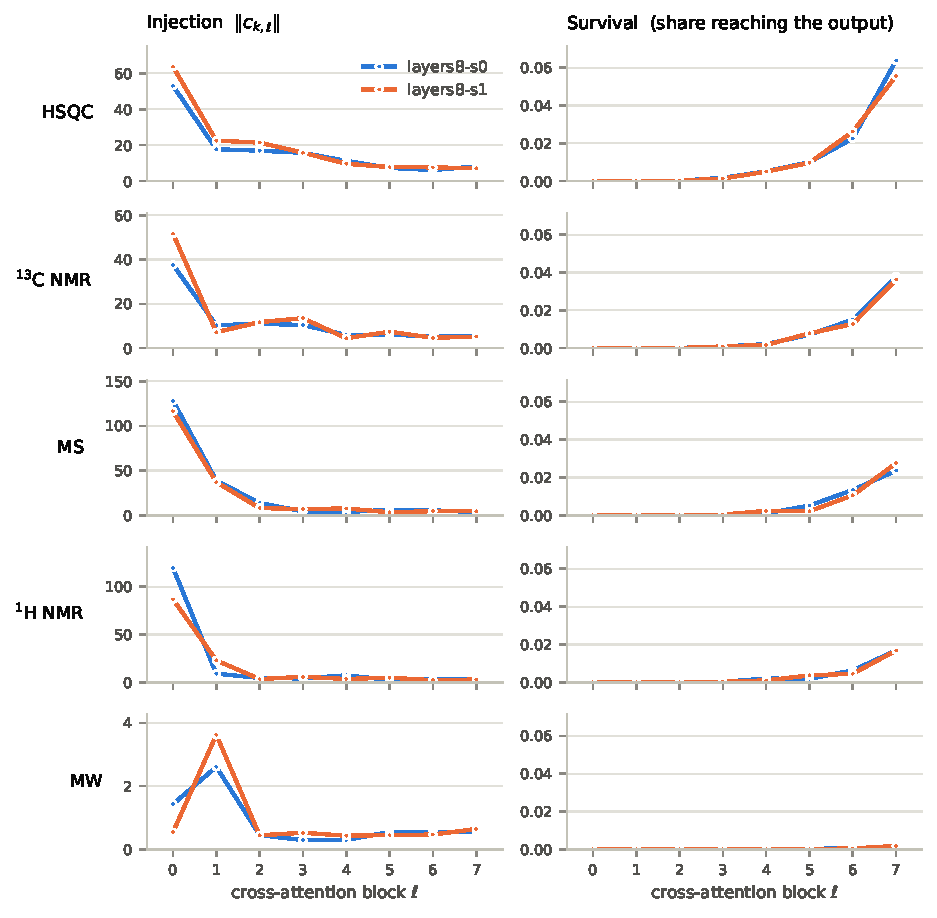
\includegraphics[width=0.92\textwidth]{fig-layer-profile-8L.pdf}
\caption{Per-block, per-modality survival and injection profile for the 8-layer
arms.}
\end{figure}

\FloatBarrier
\section{Caveats}
\label{sec:caveats}

\begin{enumerate}
  \item \textbf{Unequal sample sizes.} The 8-layer arms use $n=2048$; the
    16-layer reference uses $n=256$ (attribution) and $n=512$ (suppression).
    The 16-layer column is the noisier one, so the agreement in
    Table~\ref{tab:last} is if anything understated --- but a matched-$n$ rerun
    would make the comparison clean, and is cheap.
  \item \textbf{The 16-layer reference is not the same measurement as the
    published one.} These numbers come from \code{final1/best.ckpt} at $n=256$.
    The modality-attribution write-up quotes $9.2\times$ superadditivity and
    Spearman $1.0$ from a different run at different $n$. Both are correct for
    what they measure; quoting across them is not.
  \item \textbf{Two seeds, not three.} \code{layers8-s2} finished after these
    measurements were taken and is not included.
  \item \textbf{Suppression is not retraining.} Zeroing a block's attention
    output in a trained network measures what that block currently contributes,
    not what a network trained without it would do. The retrieval sweep is the
    experiment that answers the latter; this note explains its result.
\end{enumerate}

\section{Conclusion}

Halving MARINA's cross-attention depth does not change what the stack computes.
The live suffix is $5$--$6$ blocks either way, the cost of suppressing the last
$k$ blocks matches across depths to within $0.012$ for $k \le 4$, and the
modality budget is unchanged. The eight blocks removed from the 16-layer model
were part of an inert prefix that contributed under $0.01$ cosine in total.

This is the mechanistic reason \code{layers8} matches \code{layers12} on test
\code{rank@1}, and it predicts that further trimming would start to cost
something between six and five blocks, where the cliff sits.

\end{document}
